\documentclass[twoside]{book}

% Packages required by doxygen
\usepackage{calc}
\usepackage{doxygen}
\usepackage{graphicx}
\usepackage[utf8]{inputenc}
\usepackage{makeidx}
\usepackage{multicol}
\usepackage{multirow}
\usepackage{textcomp}
\usepackage[table]{xcolor}

% Font selection
\usepackage[T1]{fontenc}
\usepackage{mathptmx}
\usepackage[scaled=.90]{helvet}
\usepackage{courier}
\usepackage{amssymb}
\usepackage{sectsty}
\renewcommand{\familydefault}{\sfdefault}
\allsectionsfont{%
  \fontseries{bc}\selectfont%
  \color{darkgray}%
}
\renewcommand{\DoxyLabelFont}{%
  \fontseries{bc}\selectfont%
  \color{darkgray}%
}

% Page & text layout
\usepackage{geometry}
\geometry{%
  a4paper,%
  top=2.5cm,%
  bottom=2.5cm,%
  left=2.5cm,%
  right=2.5cm%
}
\tolerance=750
\hfuzz=15pt
\hbadness=750
\setlength{\emergencystretch}{15pt}
\setlength{\parindent}{0cm}
\setlength{\parskip}{0.2cm}
\makeatletter
\renewcommand{\paragraph}{%
  \@startsection{paragraph}{4}{0ex}{-1.0ex}{1.0ex}{%
    \normalfont\normalsize\bfseries\SS@parafont%
  }%
}
\renewcommand{\subparagraph}{%
  \@startsection{subparagraph}{5}{0ex}{-1.0ex}{1.0ex}{%
    \normalfont\normalsize\bfseries\SS@subparafont%
  }%
}
\makeatother

% Headers & footers
\usepackage{fancyhdr}
\pagestyle{fancyplain}
\fancyhead[LE]{\fancyplain{}{\bfseries\thepage}}
\fancyhead[CE]{\fancyplain{}{}}
\fancyhead[RE]{\fancyplain{}{\bfseries\leftmark}}
\fancyhead[LO]{\fancyplain{}{\bfseries\rightmark}}
\fancyhead[CO]{\fancyplain{}{}}
\fancyhead[RO]{\fancyplain{}{\bfseries\thepage}}
\fancyfoot[LE]{\fancyplain{}{}}
\fancyfoot[CE]{\fancyplain{}{}}
\fancyfoot[RE]{\fancyplain{}{\bfseries\scriptsize Generated on Thu Sep 12 2013 13\-:37\-:21 for Chess by Doxygen }}
\fancyfoot[LO]{\fancyplain{}{\bfseries\scriptsize Generated on Thu Sep 12 2013 13\-:37\-:21 for Chess by Doxygen }}
\fancyfoot[CO]{\fancyplain{}{}}
\fancyfoot[RO]{\fancyplain{}{}}
\renewcommand{\footrulewidth}{0.4pt}
\renewcommand{\chaptermark}[1]{%
  \markboth{#1}{}%
}
\renewcommand{\sectionmark}[1]{%
  \markright{\thesection\ #1}%
}

% Indices & bibliography
\usepackage{natbib}
\usepackage[titles]{tocloft}
\setcounter{tocdepth}{3}
\setcounter{secnumdepth}{5}
\makeindex

% Hyperlinks (required, but should be loaded last)
\usepackage{ifpdf}
\ifpdf
  \usepackage[pdftex,pagebackref=true]{hyperref}
\else
  \usepackage[ps2pdf,pagebackref=true]{hyperref}
\fi
\hypersetup{%
  colorlinks=true,%
  linkcolor=blue,%
  citecolor=blue,%
  unicode%
}

% Custom commands
\newcommand{\clearemptydoublepage}{%
  \newpage{\pagestyle{empty}\cleardoublepage}%
}


%===== C O N T E N T S =====

\begin{document}

% Titlepage & ToC
\hypersetup{pageanchor=false}
\pagenumbering{roman}
\begin{titlepage}
\vspace*{7cm}
\begin{center}%
{\Large Chess }\\
\vspace*{1cm}
{\large Generated by Doxygen 1.8.5}\\
\vspace*{0.5cm}
{\small Thu Sep 12 2013 13:37:21}\\
\end{center}
\end{titlepage}
\clearemptydoublepage
\tableofcontents
\clearemptydoublepage
\pagenumbering{arabic}
\hypersetup{pageanchor=true}

%--- Begin generated contents ---
\chapter{Hierarchical Index}
\section{Class Hierarchy}
This inheritance list is sorted roughly, but not completely, alphabetically\-:\begin{DoxyCompactList}
\item \contentsline{section}{board.\-Board}{\pageref{classboard_1_1_board}}{}
\item \contentsline{section}{test.\-Board\-Test}{\pageref{classtest_1_1_board_test}}{}
\item \contentsline{section}{enums.\-Board\-Type}{\pageref{enumenums_1_1_board_type}}{}
\item \contentsline{section}{runner.\-Chess\-Game}{\pageref{classrunner_1_1_chess_game}}{}
\item \contentsline{section}{pieces.\-Piece}{\pageref{classpieces_1_1_piece}}{}
\begin{DoxyCompactList}
\item \contentsline{section}{pieces.\-Bishop}{\pageref{classpieces_1_1_bishop}}{}
\item \contentsline{section}{pieces.\-Ferz}{\pageref{classpieces_1_1_ferz}}{}
\item \contentsline{section}{pieces.\-King}{\pageref{classpieces_1_1_king}}{}
\item \contentsline{section}{pieces.\-Knight}{\pageref{classpieces_1_1_knight}}{}
\item \contentsline{section}{pieces.\-Pawn}{\pageref{classpieces_1_1_pawn}}{}
\item \contentsline{section}{pieces.\-Queen}{\pageref{classpieces_1_1_queen}}{}
\item \contentsline{section}{pieces.\-Rook}{\pageref{classpieces_1_1_rook}}{}
\item \contentsline{section}{pieces.\-Wazir}{\pageref{classpieces_1_1_wazir}}{}
\end{DoxyCompactList}
\item \contentsline{section}{Player}{\pageref{class_player}}{}
\item \contentsline{section}{board.\-Square}{\pageref{classboard_1_1_square}}{}
\item J\-Frame\begin{DoxyCompactList}
\item \contentsline{section}{gui.\-Main\-Frame}{\pageref{classgui_1_1_main_frame}}{}
\end{DoxyCompactList}
\item J\-Panel\begin{DoxyCompactList}
\item \contentsline{section}{gui.\-Classic\-Board\-Panel}{\pageref{classgui_1_1_classic_board_panel}}{}
\end{DoxyCompactList}
\end{DoxyCompactList}

\chapter{Class Index}
\section{Class List}
Here are the classes, structs, unions and interfaces with brief descriptions\-:\begin{DoxyCompactList}
\item\contentsline{section}{\hyperlink{classpieces_1_1_bishop}{pieces.\-Bishop} }{\pageref{classpieces_1_1_bishop}}{}
\item\contentsline{section}{\hyperlink{classboard_1_1_board}{board.\-Board} }{\pageref{classboard_1_1_board}}{}
\item\contentsline{section}{\hyperlink{classtest_1_1_board_test}{test.\-Board\-Test} }{\pageref{classtest_1_1_board_test}}{}
\item\contentsline{section}{\hyperlink{enumenums_1_1_board_type}{enums.\-Board\-Type} }{\pageref{enumenums_1_1_board_type}}{}
\item\contentsline{section}{\hyperlink{classrunner_1_1_chess_game}{runner.\-Chess\-Game} }{\pageref{classrunner_1_1_chess_game}}{}
\item\contentsline{section}{\hyperlink{classgui_1_1_classic_board_panel}{gui.\-Classic\-Board\-Panel} }{\pageref{classgui_1_1_classic_board_panel}}{}
\item\contentsline{section}{\hyperlink{classpieces_1_1_ferz}{pieces.\-Ferz} }{\pageref{classpieces_1_1_ferz}}{}
\item\contentsline{section}{\hyperlink{classpieces_1_1_king}{pieces.\-King} }{\pageref{classpieces_1_1_king}}{}
\item\contentsline{section}{\hyperlink{classpieces_1_1_knight}{pieces.\-Knight} }{\pageref{classpieces_1_1_knight}}{}
\item\contentsline{section}{\hyperlink{classgui_1_1_main_frame}{gui.\-Main\-Frame} }{\pageref{classgui_1_1_main_frame}}{}
\item\contentsline{section}{\hyperlink{classpieces_1_1_pawn}{pieces.\-Pawn} }{\pageref{classpieces_1_1_pawn}}{}
\item\contentsline{section}{\hyperlink{classpieces_1_1_piece}{pieces.\-Piece} }{\pageref{classpieces_1_1_piece}}{}
\item\contentsline{section}{\hyperlink{class_player}{Player} }{\pageref{class_player}}{}
\item\contentsline{section}{\hyperlink{classpieces_1_1_queen}{pieces.\-Queen} }{\pageref{classpieces_1_1_queen}}{}
\item\contentsline{section}{\hyperlink{classpieces_1_1_rook}{pieces.\-Rook} }{\pageref{classpieces_1_1_rook}}{}
\item\contentsline{section}{\hyperlink{classboard_1_1_square}{board.\-Square} }{\pageref{classboard_1_1_square}}{}
\item\contentsline{section}{\hyperlink{classpieces_1_1_wazir}{pieces.\-Wazir} }{\pageref{classpieces_1_1_wazir}}{}
\end{DoxyCompactList}

\chapter{Class Documentation}
\hypertarget{classpieces_1_1_bishop}{\section{pieces.\-Bishop Class Reference}
\label{classpieces_1_1_bishop}\index{pieces.\-Bishop@{pieces.\-Bishop}}
}
Inheritance diagram for pieces.\-Bishop\-:\begin{figure}[H]
\begin{center}
\leavevmode
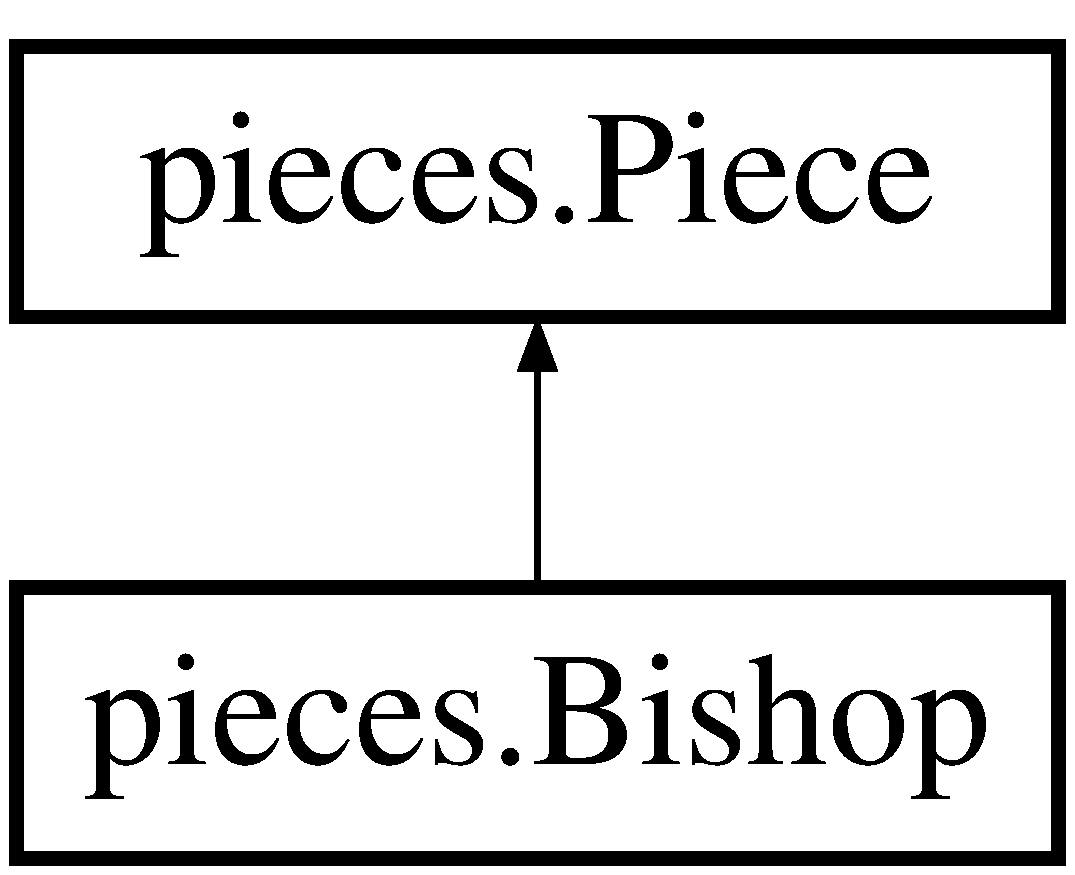
\includegraphics[height=2.000000cm]{classpieces_1_1_bishop}
\end{center}
\end{figure}
\subsection*{Public Member Functions}
\begin{DoxyCompactItemize}
\item 
\hypertarget{classpieces_1_1_bishop_a86895ed4b23625d12e5569476046a935}{{\bfseries Bishop} (Color c, int x\-Loc, int y\-Loc)}\label{classpieces_1_1_bishop_a86895ed4b23625d12e5569476046a935}

\item 
\hypertarget{classpieces_1_1_bishop_ab7a247967b43c97aa92ca28db34a9af7}{boolean {\bfseries can\-Move\-To} (\hyperlink{classboard_1_1_square}{Square} square)}\label{classpieces_1_1_bishop_ab7a247967b43c97aa92ca28db34a9af7}

\item 
\hypertarget{classpieces_1_1_bishop_ae2b131bf6057162510986844900ae7e7}{int\mbox{[}$\,$\mbox{]}\mbox{[}$\,$\mbox{]} {\bfseries get\-Path\-To} (\hyperlink{classboard_1_1_square}{Square} square)}\label{classpieces_1_1_bishop_ae2b131bf6057162510986844900ae7e7}

\end{DoxyCompactItemize}
\subsection*{Additional Inherited Members}


The documentation for this class was generated from the following file\-:\begin{DoxyCompactItemize}
\item 
src/pieces/Bishop.\-java\end{DoxyCompactItemize}

\hypertarget{classboard_1_1_board}{\section{board.\-Board Class Reference}
\label{classboard_1_1_board}\index{board.\-Board@{board.\-Board}}
}
\subsection*{Public Member Functions}
\begin{DoxyCompactItemize}
\item 
\hyperlink{classboard_1_1_board_a3dc277f7d2c22ce8d90dd98c9301371d}{Board} (int board\-Width, int board\-Height, \hyperlink{enumenums_1_1_board_type}{Board\-Type} board\-Type)
\item 
\hyperlink{classpieces_1_1_piece}{Piece} \hyperlink{classboard_1_1_board_adcfe685a47776e1aaab004b0dbdb55ee}{get\-Piece\-At} (int row, int column)
\item 
boolean \hyperlink{classboard_1_1_board_a4494901eef890f371c30e8656c5c1d77}{move} (int start\-Row, int start\-Col, int end\-Row, int end\-Col, Color player\-Color)
\item 
int \hyperlink{classboard_1_1_board_a6b17aec4022d0a4314393d246c3d48f3}{get\-Columns} ()
\item 
int \hyperlink{classboard_1_1_board_a0c300f5c0399ec83a4065663a35ac9e9}{get\-Rows} ()
\item 
\hyperlink{classboard_1_1_square}{Square}\mbox{[}$\,$\mbox{]}\mbox{[}$\,$\mbox{]} \hyperlink{classboard_1_1_board_aec5c6e50e5a17970d69809f8b87a648a}{get\-Squares} ()
\item 
\hyperlink{classboard_1_1_square}{Square} \hyperlink{classboard_1_1_board_afa9b4609be24b62dc2d9b0c69a10446b}{get\-Square} (int a\-Row, int a\-Col)
\end{DoxyCompactItemize}


\subsection{Constructor \& Destructor Documentation}
\hypertarget{classboard_1_1_board_a3dc277f7d2c22ce8d90dd98c9301371d}{\index{board\-::\-Board@{board\-::\-Board}!Board@{Board}}
\index{Board@{Board}!board::Board@{board\-::\-Board}}
\subsubsection[{Board}]{\setlength{\rightskip}{0pt plus 5cm}board.\-Board.\-Board (
\begin{DoxyParamCaption}
\item[{int}]{board\-Width, }
\item[{int}]{board\-Height, }
\item[{{\bf Board\-Type}}]{board\-Type}
\end{DoxyParamCaption}
)\hspace{0.3cm}{\ttfamily [inline]}}}\label{classboard_1_1_board_a3dc277f7d2c22ce8d90dd98c9301371d}
\hyperlink{classboard_1_1_board}{Board} -\/ Constructor 
\begin{DoxyParams}{Parameters}
{\em board\-Width} & -\/ width of the board \\
\hline
{\em board\-Height} & -\/ height of the board \\
\hline
{\em board\-Type} & -\/ type of the board setup \\
\hline
\end{DoxyParams}


\subsection{Member Function Documentation}
\hypertarget{classboard_1_1_board_a6b17aec4022d0a4314393d246c3d48f3}{\index{board\-::\-Board@{board\-::\-Board}!get\-Columns@{get\-Columns}}
\index{get\-Columns@{get\-Columns}!board::Board@{board\-::\-Board}}
\subsubsection[{get\-Columns}]{\setlength{\rightskip}{0pt plus 5cm}int board.\-Board.\-get\-Columns (
\begin{DoxyParamCaption}
{}
\end{DoxyParamCaption}
)\hspace{0.3cm}{\ttfamily [inline]}}}\label{classboard_1_1_board_a6b17aec4022d0a4314393d246c3d48f3}
\begin{DoxyReturn}{Returns}
the columns 
\end{DoxyReturn}
\hypertarget{classboard_1_1_board_adcfe685a47776e1aaab004b0dbdb55ee}{\index{board\-::\-Board@{board\-::\-Board}!get\-Piece\-At@{get\-Piece\-At}}
\index{get\-Piece\-At@{get\-Piece\-At}!board::Board@{board\-::\-Board}}
\subsubsection[{get\-Piece\-At}]{\setlength{\rightskip}{0pt plus 5cm}{\bf Piece} board.\-Board.\-get\-Piece\-At (
\begin{DoxyParamCaption}
\item[{int}]{row, }
\item[{int}]{column}
\end{DoxyParamCaption}
)\hspace{0.3cm}{\ttfamily [inline]}}}\label{classboard_1_1_board_adcfe685a47776e1aaab004b0dbdb55ee}

\begin{DoxyParams}{Parameters}
{\em row} & the row to get the piece from \\
\hline
{\em column} & the column to get the piece from \\
\hline
\end{DoxyParams}
\begin{DoxyReturn}{Returns}
returns the piece at the given location 
\end{DoxyReturn}
\hypertarget{classboard_1_1_board_a0c300f5c0399ec83a4065663a35ac9e9}{\index{board\-::\-Board@{board\-::\-Board}!get\-Rows@{get\-Rows}}
\index{get\-Rows@{get\-Rows}!board::Board@{board\-::\-Board}}
\subsubsection[{get\-Rows}]{\setlength{\rightskip}{0pt plus 5cm}int board.\-Board.\-get\-Rows (
\begin{DoxyParamCaption}
{}
\end{DoxyParamCaption}
)\hspace{0.3cm}{\ttfamily [inline]}}}\label{classboard_1_1_board_a0c300f5c0399ec83a4065663a35ac9e9}
\begin{DoxyReturn}{Returns}
the rows 
\end{DoxyReturn}
\hypertarget{classboard_1_1_board_afa9b4609be24b62dc2d9b0c69a10446b}{\index{board\-::\-Board@{board\-::\-Board}!get\-Square@{get\-Square}}
\index{get\-Square@{get\-Square}!board::Board@{board\-::\-Board}}
\subsubsection[{get\-Square}]{\setlength{\rightskip}{0pt plus 5cm}{\bf Square} board.\-Board.\-get\-Square (
\begin{DoxyParamCaption}
\item[{int}]{a\-Row, }
\item[{int}]{a\-Col}
\end{DoxyParamCaption}
)\hspace{0.3cm}{\ttfamily [inline]}}}\label{classboard_1_1_board_afa9b4609be24b62dc2d9b0c69a10446b}
\begin{DoxyReturn}{Returns}
the square at the given location, null if bad location 
\end{DoxyReturn}
\hypertarget{classboard_1_1_board_aec5c6e50e5a17970d69809f8b87a648a}{\index{board\-::\-Board@{board\-::\-Board}!get\-Squares@{get\-Squares}}
\index{get\-Squares@{get\-Squares}!board::Board@{board\-::\-Board}}
\subsubsection[{get\-Squares}]{\setlength{\rightskip}{0pt plus 5cm}{\bf Square} \mbox{[}$\,$\mbox{]}\mbox{[}$\,$\mbox{]} board.\-Board.\-get\-Squares (
\begin{DoxyParamCaption}
{}
\end{DoxyParamCaption}
)\hspace{0.3cm}{\ttfamily [inline]}}}\label{classboard_1_1_board_aec5c6e50e5a17970d69809f8b87a648a}
\begin{DoxyReturn}{Returns}
the squares 
\end{DoxyReturn}
\hypertarget{classboard_1_1_board_a4494901eef890f371c30e8656c5c1d77}{\index{board\-::\-Board@{board\-::\-Board}!move@{move}}
\index{move@{move}!board::Board@{board\-::\-Board}}
\subsubsection[{move}]{\setlength{\rightskip}{0pt plus 5cm}boolean board.\-Board.\-move (
\begin{DoxyParamCaption}
\item[{int}]{start\-Row, }
\item[{int}]{start\-Col, }
\item[{int}]{end\-Row, }
\item[{int}]{end\-Col, }
\item[{Color}]{player\-Color}
\end{DoxyParamCaption}
)\hspace{0.3cm}{\ttfamily [inline]}}}\label{classboard_1_1_board_a4494901eef890f371c30e8656c5c1d77}
move -\/ move a piece from a start square to a destination square 
\begin{DoxyParams}{Parameters}
{\em start\-Row} & -\/ the row coord of the piece to move \\
\hline
{\em start\-Col} & -\/ the column coord of the piece to move \\
\hline
{\em end\-Row} & -\/ the row coord of the square to move to \\
\hline
{\em end\-Col} & -\/ the column coord of the square to move to \\
\hline
{\em player\-Color} & -\/ the color of the player who is moving a piece \\
\hline
\end{DoxyParams}
\begin{DoxyReturn}{Returns}
true if the move was successful, false if not 
\end{DoxyReturn}


The documentation for this class was generated from the following file\-:\begin{DoxyCompactItemize}
\item 
src/board/Board.\-java\end{DoxyCompactItemize}

\hypertarget{classtest_1_1_board_test}{\section{test.\-Board\-Test Class Reference}
\label{classtest_1_1_board_test}\index{test.\-Board\-Test@{test.\-Board\-Test}}
}
\subsection*{Public Member Functions}
\begin{DoxyCompactItemize}
\item 
\hypertarget{classtest_1_1_board_test_ab34e21f215b8f4f3789e9533ba939a61}{void {\bfseries test\-Board\-Classic} ()  throws Exception }\label{classtest_1_1_board_test_ab34e21f215b8f4f3789e9533ba939a61}

\item 
\hypertarget{classtest_1_1_board_test_a4cfee6a77257f3f693a758201d4b4585}{void {\bfseries test\-Piece\-Movement\-When\-Blocked} ()}\label{classtest_1_1_board_test_a4cfee6a77257f3f693a758201d4b4585}

\item 
\hypertarget{classtest_1_1_board_test_a5556f974d1e968221a4cc965e2bf6476}{void {\bfseries test\-Piece\-Movement\-When\-Wrong\-Color} ()}\label{classtest_1_1_board_test_a5556f974d1e968221a4cc965e2bf6476}

\end{DoxyCompactItemize}


The documentation for this class was generated from the following file\-:\begin{DoxyCompactItemize}
\item 
src/test/Board\-Test.\-java\end{DoxyCompactItemize}

\hypertarget{enumenums_1_1_board_type}{\section{enums.\-Board\-Type Enum Reference}
\label{enumenums_1_1_board_type}\index{enums.\-Board\-Type@{enums.\-Board\-Type}}
}
\subsection*{Public Attributes}
\begin{DoxyCompactItemize}
\item 
\hypertarget{enumenums_1_1_board_type_a4422b8c65e5fbee0e8c19987ac5d18e6}{{\bfseries C\-L\-A\-S\-S\-I\-C}}\label{enumenums_1_1_board_type_a4422b8c65e5fbee0e8c19987ac5d18e6}

\item 
\hypertarget{enumenums_1_1_board_type_a46abe0dff948aaf03e00ca391742ac75}{{\bfseries L\-O\-N\-G}}\label{enumenums_1_1_board_type_a46abe0dff948aaf03e00ca391742ac75}

\end{DoxyCompactItemize}


The documentation for this enum was generated from the following file\-:\begin{DoxyCompactItemize}
\item 
src/enums/Board\-Type.\-java\end{DoxyCompactItemize}

\hypertarget{classrunner_1_1_chess_game}{\section{runner.\-Chess\-Game Class Reference}
\label{classrunner_1_1_chess_game}\index{runner.\-Chess\-Game@{runner.\-Chess\-Game}}
}
\subsection*{Static Public Member Functions}
\begin{DoxyCompactItemize}
\item 
\hypertarget{classrunner_1_1_chess_game_aacd962a1c3446bc4857ab3f32dbafe89}{static void {\bfseries main} (String\mbox{[}$\,$\mbox{]} args)}\label{classrunner_1_1_chess_game_aacd962a1c3446bc4857ab3f32dbafe89}

\end{DoxyCompactItemize}


The documentation for this class was generated from the following file\-:\begin{DoxyCompactItemize}
\item 
src/runner/Chess\-Game.\-java\end{DoxyCompactItemize}

\hypertarget{classgui_1_1_classic_board_panel}{\section{gui.\-Classic\-Board\-Panel Class Reference}
\label{classgui_1_1_classic_board_panel}\index{gui.\-Classic\-Board\-Panel@{gui.\-Classic\-Board\-Panel}}
}
Inheritance diagram for gui.\-Classic\-Board\-Panel\-:\begin{figure}[H]
\begin{center}
\leavevmode
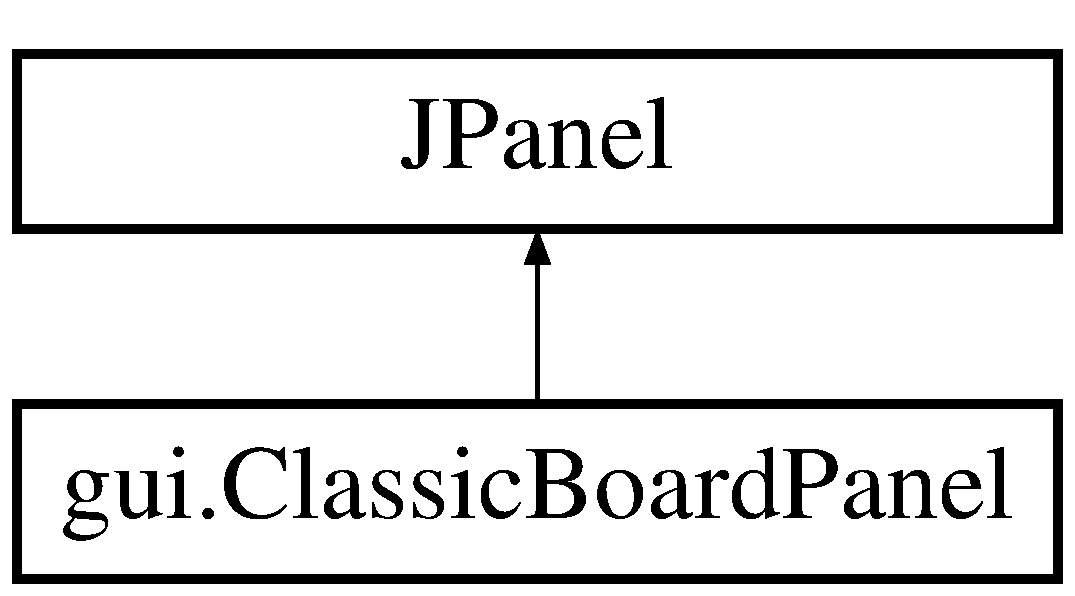
\includegraphics[height=2.000000cm]{classgui_1_1_classic_board_panel}
\end{center}
\end{figure}
\subsection*{Public Member Functions}
\begin{DoxyCompactItemize}
\item 
\hyperlink{classgui_1_1_classic_board_panel_a5d6b39fc4009b005514c9947127f097a}{Classic\-Board\-Panel} (\hyperlink{classboard_1_1_board}{Board} b)
\end{DoxyCompactItemize}


\subsection{Constructor \& Destructor Documentation}
\hypertarget{classgui_1_1_classic_board_panel_a5d6b39fc4009b005514c9947127f097a}{\index{gui\-::\-Classic\-Board\-Panel@{gui\-::\-Classic\-Board\-Panel}!Classic\-Board\-Panel@{Classic\-Board\-Panel}}
\index{Classic\-Board\-Panel@{Classic\-Board\-Panel}!gui::ClassicBoardPanel@{gui\-::\-Classic\-Board\-Panel}}
\subsubsection[{Classic\-Board\-Panel}]{\setlength{\rightskip}{0pt plus 5cm}gui.\-Classic\-Board\-Panel.\-Classic\-Board\-Panel (
\begin{DoxyParamCaption}
\item[{{\bf Board}}]{b}
\end{DoxyParamCaption}
)\hspace{0.3cm}{\ttfamily [inline]}}}\label{classgui_1_1_classic_board_panel_a5d6b39fc4009b005514c9947127f097a}
creates a panel containing the classic chess board layout 
\begin{DoxyParams}{Parameters}
{\em b} & the source board to create the graphical board from \\
\hline
\end{DoxyParams}


The documentation for this class was generated from the following file\-:\begin{DoxyCompactItemize}
\item 
src/gui/Classic\-Board\-Panel.\-java\end{DoxyCompactItemize}

\hypertarget{classpieces_1_1_ferz}{\section{pieces.\-Ferz Class Reference}
\label{classpieces_1_1_ferz}\index{pieces.\-Ferz@{pieces.\-Ferz}}
}
Inheritance diagram for pieces.\-Ferz\-:\begin{figure}[H]
\begin{center}
\leavevmode
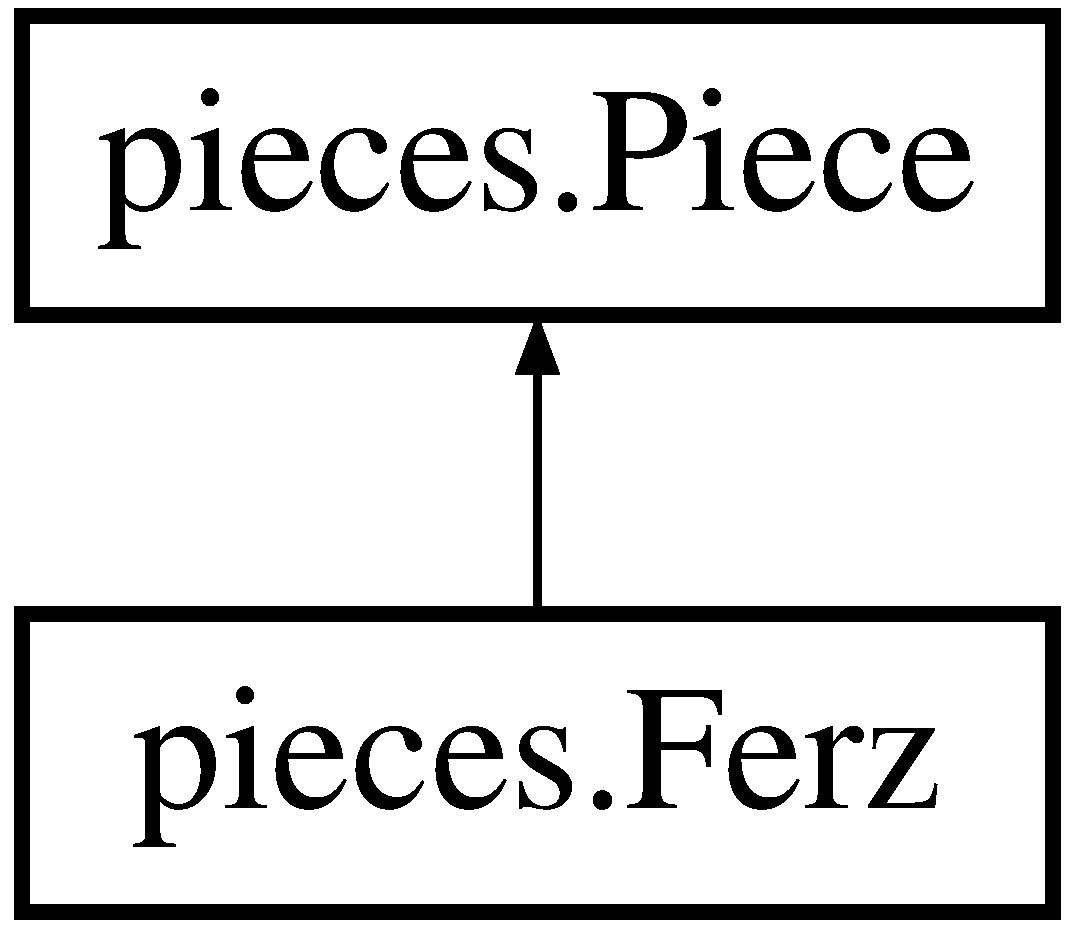
\includegraphics[height=2.000000cm]{classpieces_1_1_ferz}
\end{center}
\end{figure}
\subsection*{Public Member Functions}
\begin{DoxyCompactItemize}
\item 
\hypertarget{classpieces_1_1_ferz_a33e2c3cd35898370068ea01ab4fff6dd}{{\bfseries Ferz} (Color c, int x\-Loc, int y\-Loc)}\label{classpieces_1_1_ferz_a33e2c3cd35898370068ea01ab4fff6dd}

\item 
\hypertarget{classpieces_1_1_ferz_a2f5a851087e00b86ddf31039fec83939}{boolean {\bfseries can\-Move\-To} (\hyperlink{classboard_1_1_square}{Square} square)}\label{classpieces_1_1_ferz_a2f5a851087e00b86ddf31039fec83939}

\item 
\hypertarget{classpieces_1_1_ferz_a8b7de6969e8867d7b372a1334431f580}{int\mbox{[}$\,$\mbox{]}\mbox{[}$\,$\mbox{]} {\bfseries get\-Path\-To} (\hyperlink{classboard_1_1_square}{Square} square)}\label{classpieces_1_1_ferz_a8b7de6969e8867d7b372a1334431f580}

\end{DoxyCompactItemize}
\subsection*{Additional Inherited Members}


The documentation for this class was generated from the following file\-:\begin{DoxyCompactItemize}
\item 
src/pieces/Ferz.\-java\end{DoxyCompactItemize}

\hypertarget{classpieces_1_1_king}{\section{pieces.\-King Class Reference}
\label{classpieces_1_1_king}\index{pieces.\-King@{pieces.\-King}}
}
Inheritance diagram for pieces.\-King\-:\begin{figure}[H]
\begin{center}
\leavevmode
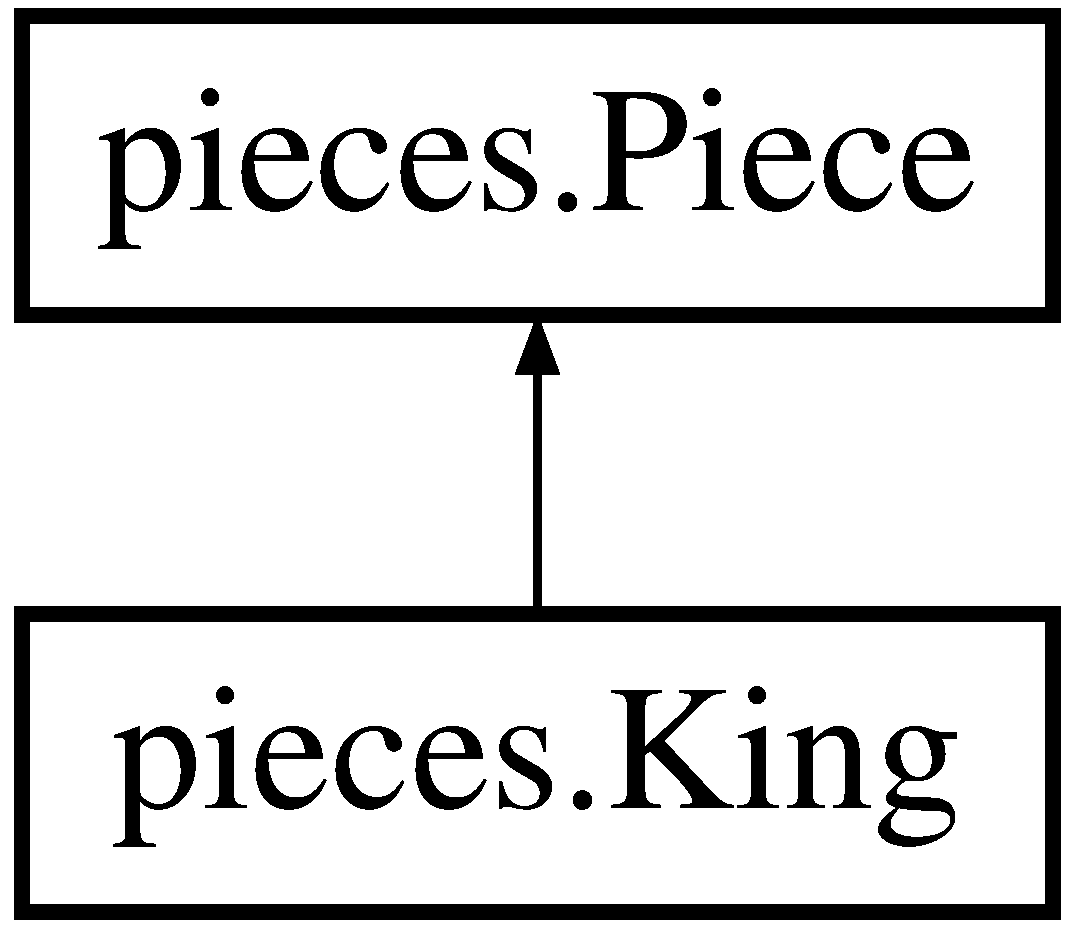
\includegraphics[height=2.000000cm]{classpieces_1_1_king}
\end{center}
\end{figure}
\subsection*{Public Member Functions}
\begin{DoxyCompactItemize}
\item 
\hypertarget{classpieces_1_1_king_aa9a279ba17536c092c053c98ff3c82c7}{{\bfseries King} (Color c, int x\-Loc, int y\-Loc)}\label{classpieces_1_1_king_aa9a279ba17536c092c053c98ff3c82c7}

\item 
\hypertarget{classpieces_1_1_king_a5288c507b0dd3c1eb0423559b6d56cc5}{boolean {\bfseries can\-Move\-To} (\hyperlink{classboard_1_1_square}{Square} square)}\label{classpieces_1_1_king_a5288c507b0dd3c1eb0423559b6d56cc5}

\item 
\hypertarget{classpieces_1_1_king_a9118974e08705ddb6723bec714c29189}{int\mbox{[}$\,$\mbox{]}\mbox{[}$\,$\mbox{]} {\bfseries get\-Path\-To} (\hyperlink{classboard_1_1_square}{Square} square)}\label{classpieces_1_1_king_a9118974e08705ddb6723bec714c29189}

\end{DoxyCompactItemize}
\subsection*{Additional Inherited Members}


The documentation for this class was generated from the following file\-:\begin{DoxyCompactItemize}
\item 
src/pieces/King.\-java\end{DoxyCompactItemize}

\hypertarget{classpieces_1_1_knight}{\section{pieces.\-Knight Class Reference}
\label{classpieces_1_1_knight}\index{pieces.\-Knight@{pieces.\-Knight}}
}
Inheritance diagram for pieces.\-Knight\-:\begin{figure}[H]
\begin{center}
\leavevmode
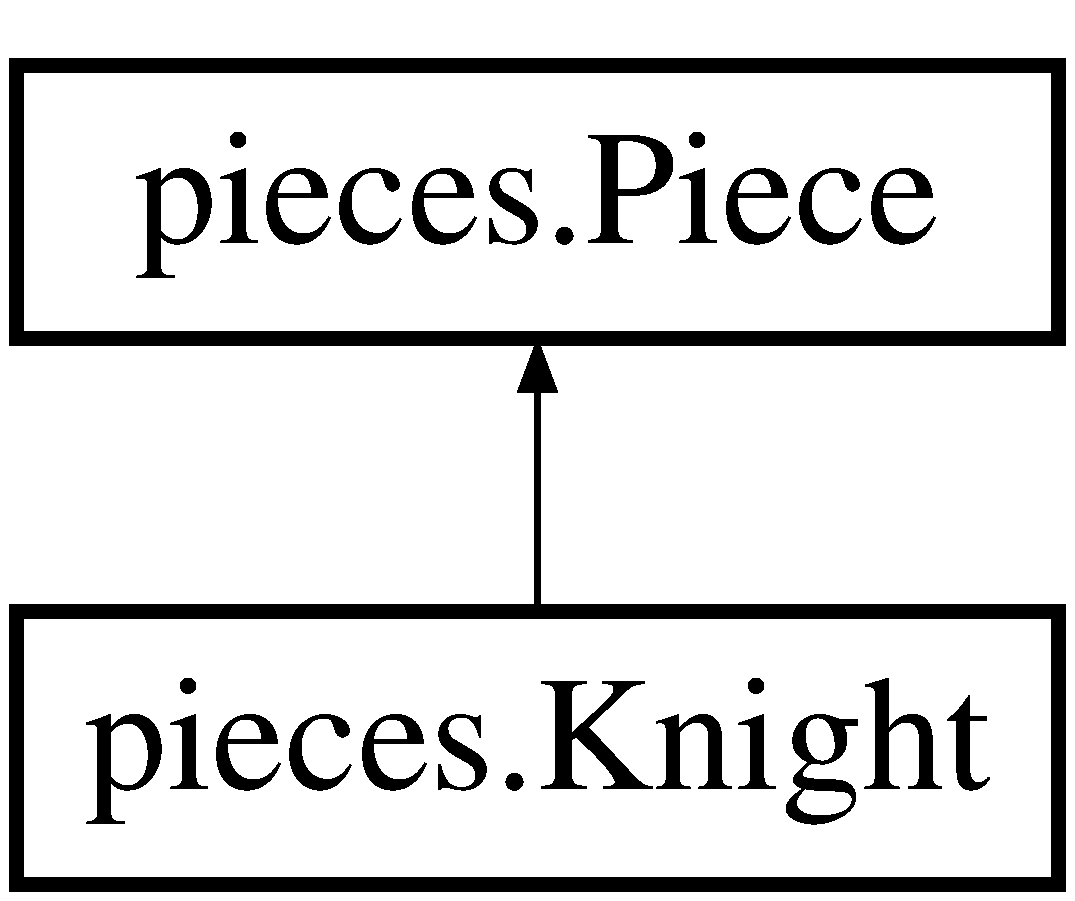
\includegraphics[height=2.000000cm]{classpieces_1_1_knight}
\end{center}
\end{figure}
\subsection*{Public Member Functions}
\begin{DoxyCompactItemize}
\item 
\hypertarget{classpieces_1_1_knight_a719936d8ccacb4e23155c646a2623614}{{\bfseries Knight} (Color c, int x\-Loc, int y\-Loc)}\label{classpieces_1_1_knight_a719936d8ccacb4e23155c646a2623614}

\item 
\hypertarget{classpieces_1_1_knight_adad62bdafec0fb68d0d05d3c44663b9e}{boolean {\bfseries can\-Move\-To} (\hyperlink{classboard_1_1_square}{Square} square)}\label{classpieces_1_1_knight_adad62bdafec0fb68d0d05d3c44663b9e}

\item 
\hypertarget{classpieces_1_1_knight_af778d7c9168b1d9f3519b98a8003a012}{int\mbox{[}$\,$\mbox{]}\mbox{[}$\,$\mbox{]} {\bfseries get\-Path\-To} (\hyperlink{classboard_1_1_square}{Square} square)}\label{classpieces_1_1_knight_af778d7c9168b1d9f3519b98a8003a012}

\end{DoxyCompactItemize}
\subsection*{Additional Inherited Members}


The documentation for this class was generated from the following file\-:\begin{DoxyCompactItemize}
\item 
src/pieces/Knight.\-java\end{DoxyCompactItemize}

\hypertarget{classgui_1_1_main_frame}{\section{gui.\-Main\-Frame Class Reference}
\label{classgui_1_1_main_frame}\index{gui.\-Main\-Frame@{gui.\-Main\-Frame}}
}
Inheritance diagram for gui.\-Main\-Frame\-:\begin{figure}[H]
\begin{center}
\leavevmode
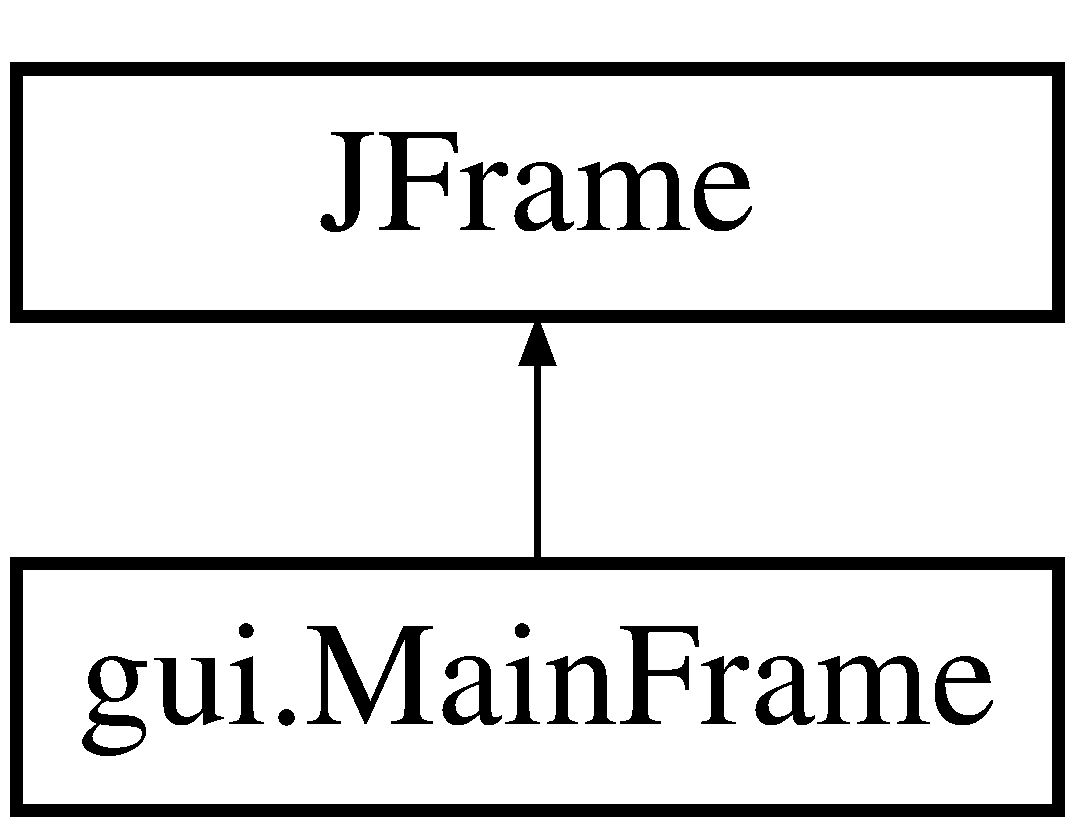
\includegraphics[height=2.000000cm]{classgui_1_1_main_frame}
\end{center}
\end{figure}
\subsection*{Public Member Functions}
\begin{DoxyCompactItemize}
\item 
\hyperlink{classgui_1_1_main_frame_a23501298b3755db8403f03632faa0271}{Main\-Frame} (\hyperlink{classboard_1_1_board}{Board} b, \hyperlink{enumenums_1_1_board_type}{Board\-Type} type)
\end{DoxyCompactItemize}


\subsection{Constructor \& Destructor Documentation}
\hypertarget{classgui_1_1_main_frame_a23501298b3755db8403f03632faa0271}{\index{gui\-::\-Main\-Frame@{gui\-::\-Main\-Frame}!Main\-Frame@{Main\-Frame}}
\index{Main\-Frame@{Main\-Frame}!gui::MainFrame@{gui\-::\-Main\-Frame}}
\subsubsection[{Main\-Frame}]{\setlength{\rightskip}{0pt plus 5cm}gui.\-Main\-Frame.\-Main\-Frame (
\begin{DoxyParamCaption}
\item[{{\bf Board}}]{b, }
\item[{{\bf Board\-Type}}]{type}
\end{DoxyParamCaption}
)\hspace{0.3cm}{\ttfamily [inline]}}}\label{classgui_1_1_main_frame_a23501298b3755db8403f03632faa0271}
Sets up the frame and adds the menu and main panel 
\begin{DoxyParams}{Parameters}
{\em b} & the board to create the gui from \\
\hline
{\em type} & the type of board layout to create the game for \\
\hline
\end{DoxyParams}


The documentation for this class was generated from the following file\-:\begin{DoxyCompactItemize}
\item 
src/gui/Main\-Frame.\-java\end{DoxyCompactItemize}

\hypertarget{classpieces_1_1_pawn}{\section{pieces.\-Pawn Class Reference}
\label{classpieces_1_1_pawn}\index{pieces.\-Pawn@{pieces.\-Pawn}}
}
Inheritance diagram for pieces.\-Pawn\-:\begin{figure}[H]
\begin{center}
\leavevmode
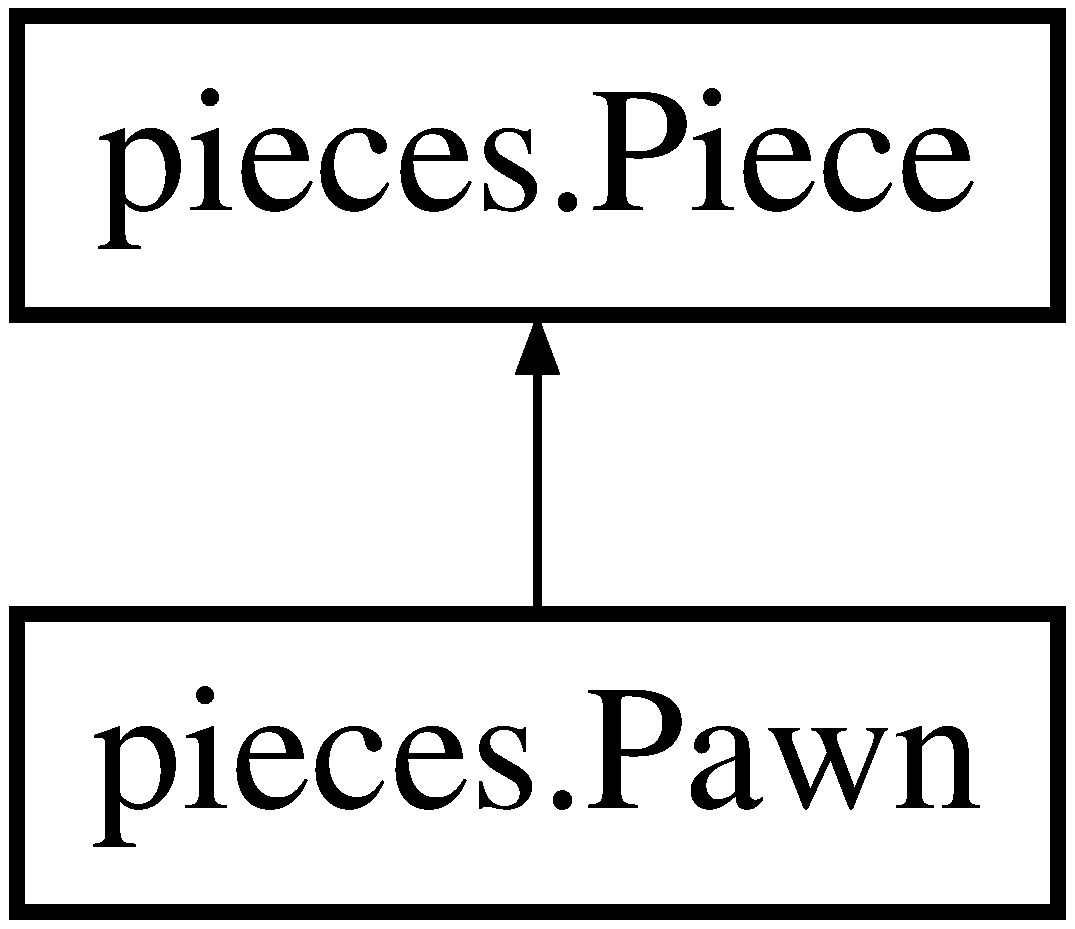
\includegraphics[height=2.000000cm]{classpieces_1_1_pawn}
\end{center}
\end{figure}
\subsection*{Public Member Functions}
\begin{DoxyCompactItemize}
\item 
\hypertarget{classpieces_1_1_pawn_a3b6bf1360b83a9b3e110fbda08aa7ea6}{{\bfseries Pawn} (Color c, int x\-Loc, int y\-Loc)}\label{classpieces_1_1_pawn_a3b6bf1360b83a9b3e110fbda08aa7ea6}

\item 
\hypertarget{classpieces_1_1_pawn_ac970afade564581d65c232f937d39988}{boolean {\bfseries can\-Move\-To} (\hyperlink{classboard_1_1_square}{Square} square)}\label{classpieces_1_1_pawn_ac970afade564581d65c232f937d39988}

\item 
\hypertarget{classpieces_1_1_pawn_a5a65d033ba2d39dd634815d5613a50b8}{boolean {\bfseries can\-Move\-First\-Turn\-To} (\hyperlink{classboard_1_1_square}{Square} square)}\label{classpieces_1_1_pawn_a5a65d033ba2d39dd634815d5613a50b8}

\item 
\hypertarget{classpieces_1_1_pawn_a929000a81247e277fcd03c9f81f4fea2}{int\mbox{[}$\,$\mbox{]}\mbox{[}$\,$\mbox{]} {\bfseries get\-Path\-To} (\hyperlink{classboard_1_1_square}{Square} square)}\label{classpieces_1_1_pawn_a929000a81247e277fcd03c9f81f4fea2}

\end{DoxyCompactItemize}
\subsection*{Additional Inherited Members}


The documentation for this class was generated from the following file\-:\begin{DoxyCompactItemize}
\item 
src/pieces/Pawn.\-java\end{DoxyCompactItemize}

\hypertarget{classpieces_1_1_piece}{\section{pieces.\-Piece Class Reference}
\label{classpieces_1_1_piece}\index{pieces.\-Piece@{pieces.\-Piece}}
}
Inheritance diagram for pieces.\-Piece\-:\begin{figure}[H]
\begin{center}
\leavevmode
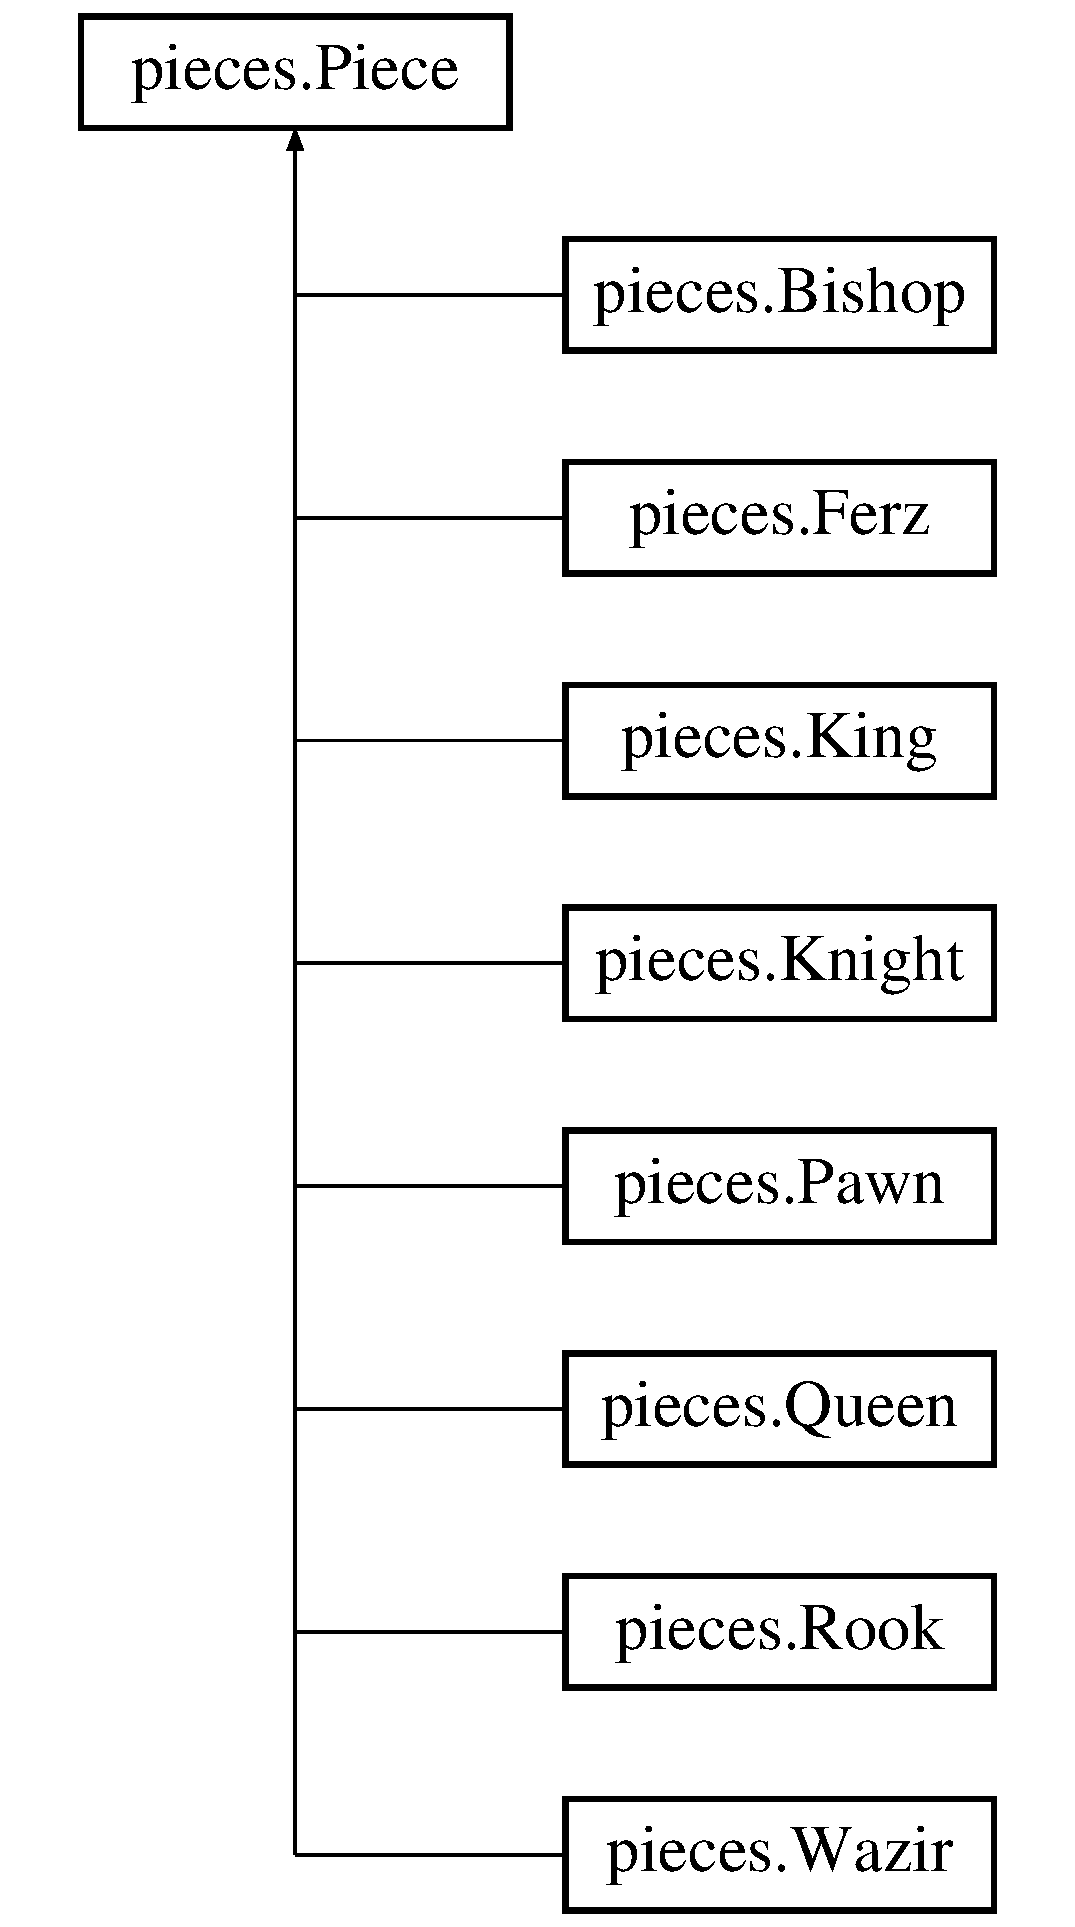
\includegraphics[height=9.000000cm]{classpieces_1_1_piece}
\end{center}
\end{figure}
\subsection*{Public Member Functions}
\begin{DoxyCompactItemize}
\item 
\hypertarget{classpieces_1_1_piece_a3bb9b8ef92de80a7ba2a1b46c188e552}{{\bfseries Piece} (Color c, int row\-Loc, int column\-Loc)}\label{classpieces_1_1_piece_a3bb9b8ef92de80a7ba2a1b46c188e552}

\item 
\hypertarget{classpieces_1_1_piece_a31ba4f2e8461b29b69bad354126ec8ad}{abstract boolean {\bfseries can\-Move\-To} (\hyperlink{classboard_1_1_square}{Square} square)}\label{classpieces_1_1_piece_a31ba4f2e8461b29b69bad354126ec8ad}

\item 
\hypertarget{classpieces_1_1_piece_aed292dabab3719b6e1ff3e83e1341047}{abstract int\mbox{[}$\,$\mbox{]}\mbox{[}$\,$\mbox{]} {\bfseries get\-Path\-To} (\hyperlink{classboard_1_1_square}{Square} square)}\label{classpieces_1_1_piece_aed292dabab3719b6e1ff3e83e1341047}

\item 
\hypertarget{classpieces_1_1_piece_aee0fc5fa7074b129aaf1f350ac8a7f1b}{Color {\bfseries get\-Color} ()}\label{classpieces_1_1_piece_aee0fc5fa7074b129aaf1f350ac8a7f1b}

\item 
\hypertarget{classpieces_1_1_piece_a61c97241febc23f209e8b70a65e02189}{void {\bfseries move\-To} (\hyperlink{classboard_1_1_square}{Square} square)}\label{classpieces_1_1_piece_a61c97241febc23f209e8b70a65e02189}

\item 
\hypertarget{classpieces_1_1_piece_a5fa8fb1fbb8509680f9fb8248897443c}{boolean {\bfseries has\-Piece\-Of\-Same\-Color} (\hyperlink{classboard_1_1_square}{Square} square)}\label{classpieces_1_1_piece_a5fa8fb1fbb8509680f9fb8248897443c}

\item 
\hypertarget{classpieces_1_1_piece_ae56bed33c272c58a382a3cc936c5806a}{boolean {\bfseries is\-Same\-Square} (\hyperlink{classboard_1_1_square}{Square} square)}\label{classpieces_1_1_piece_ae56bed33c272c58a382a3cc936c5806a}

\end{DoxyCompactItemize}
\subsection*{Public Attributes}
\begin{DoxyCompactItemize}
\item 
\hypertarget{classpieces_1_1_piece_af15165006fef783244e8bef655469461}{int {\bfseries row}}\label{classpieces_1_1_piece_af15165006fef783244e8bef655469461}

\item 
\hypertarget{classpieces_1_1_piece_a0ae0eab94abd774120ee8a26321d143f}{int {\bfseries column}}\label{classpieces_1_1_piece_a0ae0eab94abd774120ee8a26321d143f}

\item 
\hypertarget{classpieces_1_1_piece_aad2c2ef830902ae3d7da9709976216d6}{Color {\bfseries color}}\label{classpieces_1_1_piece_aad2c2ef830902ae3d7da9709976216d6}

\end{DoxyCompactItemize}


The documentation for this class was generated from the following file\-:\begin{DoxyCompactItemize}
\item 
src/pieces/Piece.\-java\end{DoxyCompactItemize}

\hypertarget{class_player}{\section{Player Class Reference}
\label{class_player}\index{Player@{Player}}
}
\subsection*{Public Member Functions}
\begin{DoxyCompactItemize}
\item 
Color \hyperlink{class_player_a19d5ea1983af3abfec99ce6a102865a1}{get\-Color} ()
\item 
void \hyperlink{class_player_a4ad5dc71ee38dbc7158951f267ec1596}{set\-Color} (Color color)
\item 
\hypertarget{class_player_afed055ca8140c2672088525f50095305}{{\bfseries Player} (Color c)}\label{class_player_afed055ca8140c2672088525f50095305}

\end{DoxyCompactItemize}


\subsection{Member Function Documentation}
\hypertarget{class_player_a19d5ea1983af3abfec99ce6a102865a1}{\index{Player@{Player}!get\-Color@{get\-Color}}
\index{get\-Color@{get\-Color}!Player@{Player}}
\subsubsection[{get\-Color}]{\setlength{\rightskip}{0pt plus 5cm}Color Player.\-get\-Color (
\begin{DoxyParamCaption}
{}
\end{DoxyParamCaption}
)\hspace{0.3cm}{\ttfamily [inline]}}}\label{class_player_a19d5ea1983af3abfec99ce6a102865a1}
\begin{DoxyReturn}{Returns}
the color 
\end{DoxyReturn}
\hypertarget{class_player_a4ad5dc71ee38dbc7158951f267ec1596}{\index{Player@{Player}!set\-Color@{set\-Color}}
\index{set\-Color@{set\-Color}!Player@{Player}}
\subsubsection[{set\-Color}]{\setlength{\rightskip}{0pt plus 5cm}void Player.\-set\-Color (
\begin{DoxyParamCaption}
\item[{Color}]{color}
\end{DoxyParamCaption}
)\hspace{0.3cm}{\ttfamily [inline]}}}\label{class_player_a4ad5dc71ee38dbc7158951f267ec1596}

\begin{DoxyParams}{Parameters}
{\em color} & the color to set \\
\hline
\end{DoxyParams}


The documentation for this class was generated from the following file\-:\begin{DoxyCompactItemize}
\item 
src/Player.\-java\end{DoxyCompactItemize}

\hypertarget{classpieces_1_1_queen}{\section{pieces.\-Queen Class Reference}
\label{classpieces_1_1_queen}\index{pieces.\-Queen@{pieces.\-Queen}}
}
Inheritance diagram for pieces.\-Queen\-:\begin{figure}[H]
\begin{center}
\leavevmode
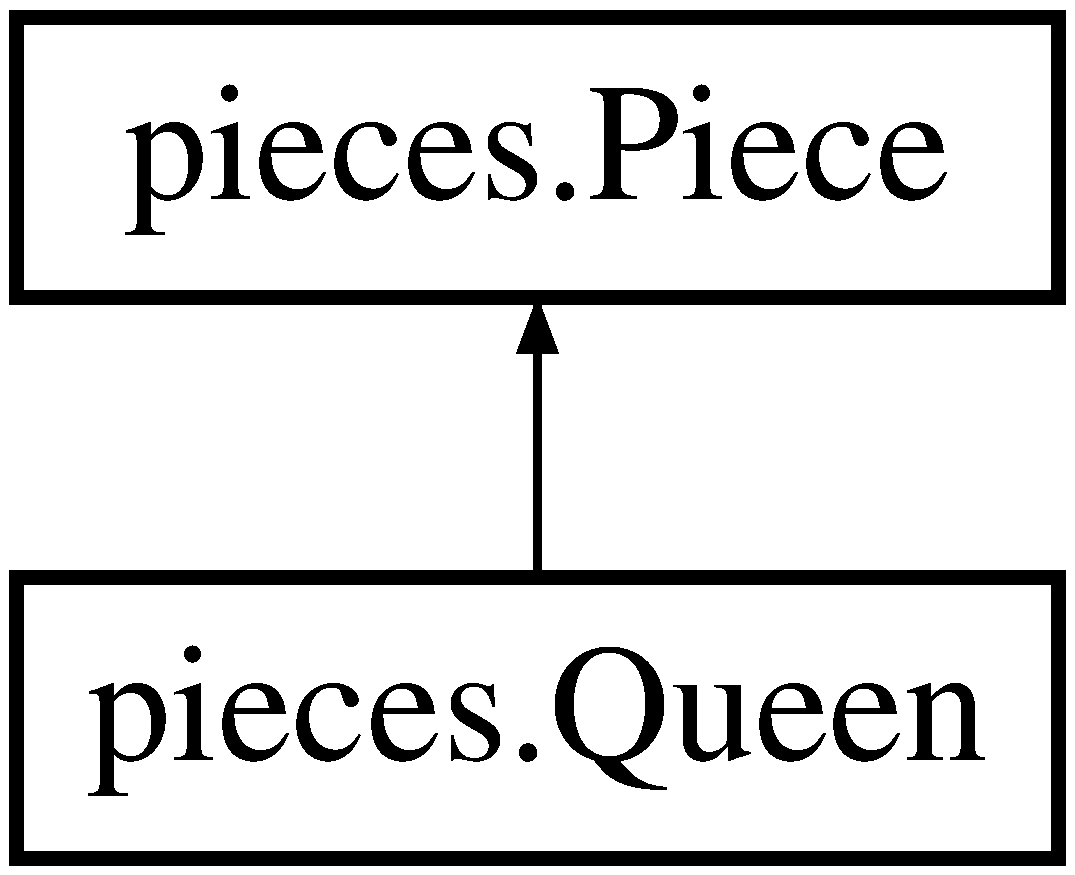
\includegraphics[height=2.000000cm]{classpieces_1_1_queen}
\end{center}
\end{figure}
\subsection*{Public Member Functions}
\begin{DoxyCompactItemize}
\item 
\hypertarget{classpieces_1_1_queen_aa5762e91511816d25d350436976ba7c7}{{\bfseries Queen} (Color c, int x\-Loc, int y\-Loc)}\label{classpieces_1_1_queen_aa5762e91511816d25d350436976ba7c7}

\item 
\hypertarget{classpieces_1_1_queen_a8dc3ad565ab37e8c006906a90024061f}{boolean {\bfseries can\-Move\-To} (\hyperlink{classboard_1_1_square}{Square} square)}\label{classpieces_1_1_queen_a8dc3ad565ab37e8c006906a90024061f}

\item 
\hypertarget{classpieces_1_1_queen_af73e59003745d9ee4055de6925cdc241}{int\mbox{[}$\,$\mbox{]}\mbox{[}$\,$\mbox{]} {\bfseries get\-Path\-To} (\hyperlink{classboard_1_1_square}{Square} square)}\label{classpieces_1_1_queen_af73e59003745d9ee4055de6925cdc241}

\end{DoxyCompactItemize}
\subsection*{Additional Inherited Members}


The documentation for this class was generated from the following file\-:\begin{DoxyCompactItemize}
\item 
src/pieces/Queen.\-java\end{DoxyCompactItemize}

\hypertarget{classpieces_1_1_rook}{\section{pieces.\-Rook Class Reference}
\label{classpieces_1_1_rook}\index{pieces.\-Rook@{pieces.\-Rook}}
}
Inheritance diagram for pieces.\-Rook\-:\begin{figure}[H]
\begin{center}
\leavevmode
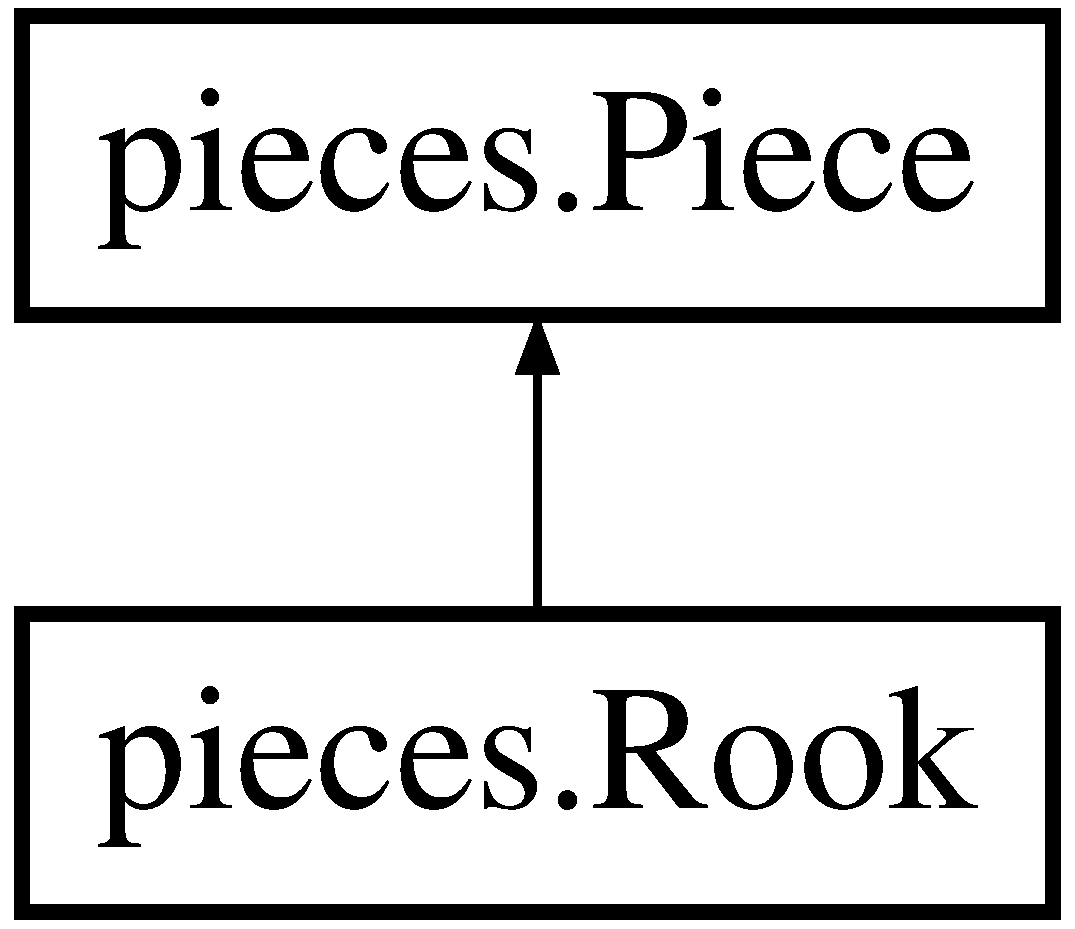
\includegraphics[height=2.000000cm]{classpieces_1_1_rook}
\end{center}
\end{figure}
\subsection*{Public Member Functions}
\begin{DoxyCompactItemize}
\item 
\hypertarget{classpieces_1_1_rook_aac55effaafd5bff2904541a0ed320d8a}{{\bfseries Rook} (Color c, int row, int column)}\label{classpieces_1_1_rook_aac55effaafd5bff2904541a0ed320d8a}

\item 
\hypertarget{classpieces_1_1_rook_a2d18bcef73cd0c629d32add4a47b96e2}{boolean {\bfseries can\-Move\-To} (\hyperlink{classboard_1_1_square}{Square} square)}\label{classpieces_1_1_rook_a2d18bcef73cd0c629d32add4a47b96e2}

\item 
\hypertarget{classpieces_1_1_rook_a51bd87b82a1c6c797a4acca806962777}{int\mbox{[}$\,$\mbox{]}\mbox{[}$\,$\mbox{]} {\bfseries get\-Path\-To} (\hyperlink{classboard_1_1_square}{Square} square)}\label{classpieces_1_1_rook_a51bd87b82a1c6c797a4acca806962777}

\end{DoxyCompactItemize}
\subsection*{Additional Inherited Members}


The documentation for this class was generated from the following file\-:\begin{DoxyCompactItemize}
\item 
src/pieces/Rook.\-java\end{DoxyCompactItemize}

\hypertarget{classboard_1_1_square}{\section{board.\-Square Class Reference}
\label{classboard_1_1_square}\index{board.\-Square@{board.\-Square}}
}
\subsection*{Public Member Functions}
\begin{DoxyCompactItemize}
\item 
\hypertarget{classboard_1_1_square_a6a23d51e6488455deca3777169fd40a4}{{\bfseries Square} (int row\-Num, int column\-Num, Color c, boolean valid)}\label{classboard_1_1_square_a6a23d51e6488455deca3777169fd40a4}

\item 
\hypertarget{classboard_1_1_square_aa174e0f9b97da735ff6a152887eab0f8}{{\bfseries Square} (int row\-Num, int column\-Num, Color c, \hyperlink{classpieces_1_1_piece}{Piece} board\-Piece)}\label{classboard_1_1_square_aa174e0f9b97da735ff6a152887eab0f8}

\item 
\hypertarget{classboard_1_1_square_ad4ad301ca32b84efe682387a9d9a319d}{boolean {\bfseries has\-Piece} ()}\label{classboard_1_1_square_ad4ad301ca32b84efe682387a9d9a319d}

\item 
\hypertarget{classboard_1_1_square_adc34c9562b336ed5c72c149fb1c9d699}{\hyperlink{classpieces_1_1_piece}{Piece} {\bfseries get\-Piece} ()}\label{classboard_1_1_square_adc34c9562b336ed5c72c149fb1c9d699}

\item 
\hypertarget{classboard_1_1_square_a0941391ade5f582b9bd70656332d6c6c}{void {\bfseries set\-Piece} (\hyperlink{classpieces_1_1_piece}{Piece} board\-Piece)}\label{classboard_1_1_square_a0941391ade5f582b9bd70656332d6c6c}

\item 
boolean \hyperlink{classboard_1_1_square_ac4361e31669bf7fb09c9d7f2945c80c0}{is\-Valid\-Space} ()
\item 
void \hyperlink{classboard_1_1_square_aaf2bb85bbd8bd7662833c477bd34a6b2}{set\-Valid\-Space} (boolean valid\-Space)
\item 
int \hyperlink{classboard_1_1_square_a6494b2e4d6e3f8c58cdbc831ce3bd161}{get\-Row} ()
\item 
int \hyperlink{classboard_1_1_square_a5b8f33f9a2e9128a734e491697059c3f}{get\-Column} ()
\item 
Color \hyperlink{classboard_1_1_square_a5e25028bc63643ff36f5b259b74adba4}{get\-Color} ()
\item 
void \hyperlink{classboard_1_1_square_a6adc448bc6c734eee3076d3b87d57930}{set\-Color} (Color color)
\end{DoxyCompactItemize}


\subsection{Member Function Documentation}
\hypertarget{classboard_1_1_square_a5e25028bc63643ff36f5b259b74adba4}{\index{board\-::\-Square@{board\-::\-Square}!get\-Color@{get\-Color}}
\index{get\-Color@{get\-Color}!board::Square@{board\-::\-Square}}
\subsubsection[{get\-Color}]{\setlength{\rightskip}{0pt plus 5cm}Color board.\-Square.\-get\-Color (
\begin{DoxyParamCaption}
{}
\end{DoxyParamCaption}
)\hspace{0.3cm}{\ttfamily [inline]}}}\label{classboard_1_1_square_a5e25028bc63643ff36f5b259b74adba4}
\begin{DoxyReturn}{Returns}
the color 
\end{DoxyReturn}
\hypertarget{classboard_1_1_square_a5b8f33f9a2e9128a734e491697059c3f}{\index{board\-::\-Square@{board\-::\-Square}!get\-Column@{get\-Column}}
\index{get\-Column@{get\-Column}!board::Square@{board\-::\-Square}}
\subsubsection[{get\-Column}]{\setlength{\rightskip}{0pt plus 5cm}int board.\-Square.\-get\-Column (
\begin{DoxyParamCaption}
{}
\end{DoxyParamCaption}
)\hspace{0.3cm}{\ttfamily [inline]}}}\label{classboard_1_1_square_a5b8f33f9a2e9128a734e491697059c3f}
\begin{DoxyReturn}{Returns}
the column 
\end{DoxyReturn}
\hypertarget{classboard_1_1_square_a6494b2e4d6e3f8c58cdbc831ce3bd161}{\index{board\-::\-Square@{board\-::\-Square}!get\-Row@{get\-Row}}
\index{get\-Row@{get\-Row}!board::Square@{board\-::\-Square}}
\subsubsection[{get\-Row}]{\setlength{\rightskip}{0pt plus 5cm}int board.\-Square.\-get\-Row (
\begin{DoxyParamCaption}
{}
\end{DoxyParamCaption}
)\hspace{0.3cm}{\ttfamily [inline]}}}\label{classboard_1_1_square_a6494b2e4d6e3f8c58cdbc831ce3bd161}
\begin{DoxyReturn}{Returns}
the row 
\end{DoxyReturn}
\hypertarget{classboard_1_1_square_ac4361e31669bf7fb09c9d7f2945c80c0}{\index{board\-::\-Square@{board\-::\-Square}!is\-Valid\-Space@{is\-Valid\-Space}}
\index{is\-Valid\-Space@{is\-Valid\-Space}!board::Square@{board\-::\-Square}}
\subsubsection[{is\-Valid\-Space}]{\setlength{\rightskip}{0pt plus 5cm}boolean board.\-Square.\-is\-Valid\-Space (
\begin{DoxyParamCaption}
{}
\end{DoxyParamCaption}
)\hspace{0.3cm}{\ttfamily [inline]}}}\label{classboard_1_1_square_ac4361e31669bf7fb09c9d7f2945c80c0}
\begin{DoxyReturn}{Returns}
the valid\-Space 
\end{DoxyReturn}
\hypertarget{classboard_1_1_square_a6adc448bc6c734eee3076d3b87d57930}{\index{board\-::\-Square@{board\-::\-Square}!set\-Color@{set\-Color}}
\index{set\-Color@{set\-Color}!board::Square@{board\-::\-Square}}
\subsubsection[{set\-Color}]{\setlength{\rightskip}{0pt plus 5cm}void board.\-Square.\-set\-Color (
\begin{DoxyParamCaption}
\item[{Color}]{color}
\end{DoxyParamCaption}
)\hspace{0.3cm}{\ttfamily [inline]}}}\label{classboard_1_1_square_a6adc448bc6c734eee3076d3b87d57930}

\begin{DoxyParams}{Parameters}
{\em color} & the color to set \\
\hline
\end{DoxyParams}
\hypertarget{classboard_1_1_square_aaf2bb85bbd8bd7662833c477bd34a6b2}{\index{board\-::\-Square@{board\-::\-Square}!set\-Valid\-Space@{set\-Valid\-Space}}
\index{set\-Valid\-Space@{set\-Valid\-Space}!board::Square@{board\-::\-Square}}
\subsubsection[{set\-Valid\-Space}]{\setlength{\rightskip}{0pt plus 5cm}void board.\-Square.\-set\-Valid\-Space (
\begin{DoxyParamCaption}
\item[{boolean}]{valid\-Space}
\end{DoxyParamCaption}
)\hspace{0.3cm}{\ttfamily [inline]}}}\label{classboard_1_1_square_aaf2bb85bbd8bd7662833c477bd34a6b2}

\begin{DoxyParams}{Parameters}
{\em valid\-Space} & set whether square is valid \\
\hline
\end{DoxyParams}


The documentation for this class was generated from the following file\-:\begin{DoxyCompactItemize}
\item 
src/board/Square.\-java\end{DoxyCompactItemize}

\hypertarget{classpieces_1_1_wazir}{\section{pieces.\-Wazir Class Reference}
\label{classpieces_1_1_wazir}\index{pieces.\-Wazir@{pieces.\-Wazir}}
}
Inheritance diagram for pieces.\-Wazir\-:\begin{figure}[H]
\begin{center}
\leavevmode
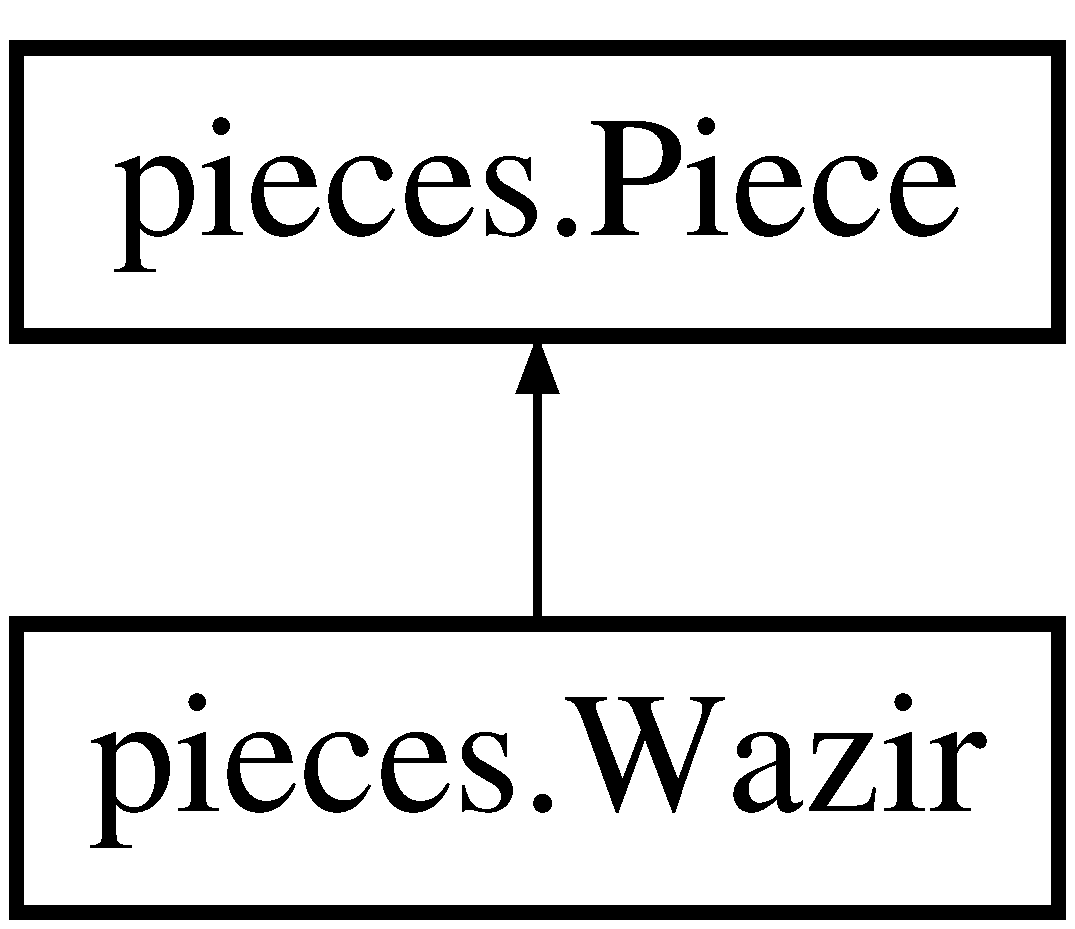
\includegraphics[height=2.000000cm]{classpieces_1_1_wazir}
\end{center}
\end{figure}
\subsection*{Public Member Functions}
\begin{DoxyCompactItemize}
\item 
\hypertarget{classpieces_1_1_wazir_a69018ccd9e05deef3f28ed5549b0bced}{{\bfseries Wazir} (Color c, int x\-Loc, int y\-Loc)}\label{classpieces_1_1_wazir_a69018ccd9e05deef3f28ed5549b0bced}

\item 
\hypertarget{classpieces_1_1_wazir_a89e055407799273ecd95f46983573663}{boolean {\bfseries can\-Move\-To} (\hyperlink{classboard_1_1_square}{Square} square)}\label{classpieces_1_1_wazir_a89e055407799273ecd95f46983573663}

\item 
\hypertarget{classpieces_1_1_wazir_a7591bea4941b3cddbcd5d5f3e94234b8}{int\mbox{[}$\,$\mbox{]}\mbox{[}$\,$\mbox{]} {\bfseries get\-Path\-To} (\hyperlink{classboard_1_1_square}{Square} square)}\label{classpieces_1_1_wazir_a7591bea4941b3cddbcd5d5f3e94234b8}

\end{DoxyCompactItemize}
\subsection*{Additional Inherited Members}


The documentation for this class was generated from the following file\-:\begin{DoxyCompactItemize}
\item 
src/pieces/Wazir.\-java\end{DoxyCompactItemize}

%--- End generated contents ---

% Index
\newpage
\phantomsection
\addcontentsline{toc}{part}{Index}
\printindex

\end{document}
